\documentclass[hyperref]{ctexart}
\usepackage[left=2.50cm, right=2.50cm, top=2.50cm, bottom=2.50cm]{geometry} %页边距
\usepackage{helvet}
\usepackage{amsmath, amsfonts, amssymb} % 数学公式、符号
\usepackage[english]{babel}
\usepackage{graphicx}   % 图片
\usepackage{url}        % 超链接
\usepackage{bm}         % 加粗方程字体
\usepackage{multirow}%合并单元格
\usepackage{booktabs}
\usepackage{algorithm}
\usepackage{algorithmic}
\usepackage{appendix}
\renewcommand{\algorithmicrequire}{ \textbf{Input:}}       
\renewcommand{\algorithmicensure}{ \textbf{Initialize:}} 
\renewcommand{\algorithmicreturn}{ \textbf{Output:}}     
%算法格式
\usepackage{listings}
\usepackage{textcomp} % 必须加上,否则报错
\usepackage[framed,numbered,autolinebreaks,useliterate]{mcode}   % 添加matlab代码宏
  \usepackage{xcolor}
  \lstset{breaklines=true} %对过长的代码自动换行
\usepackage{fancyhdr} %设置页眉、页脚
\pagestyle{fancy}
\lhead{}
\chead{}
\lfoot{}
\cfoot{}
\rfoot{}
\usepackage{hyperref} %bookmarks
\hypersetup{colorlinks, bookmarks, unicode} %unicode
\usepackage{multicol}
\title{\textbf{图像重建的数学方法}}
\author{\sffamily 苏学睿$^1$}
\date{(Dated: \today)}
\begin{document}
	\maketitle
		\noindent{\bf Abstract: }

			$CT$技术是一种先进的可视化技术,是核物理、核电子学、精密机械和计算机科学相结合而产生的一门新的成像技术,被国际无损检测界公认为最佳无损检测手段。$CT$成像的原理是由投影重建图像的理论。自从1917年$Radon$提出了著名的$Radon$变换,该理论就成为$CT$重建技术的重要基础。图像重建算法主要方法分为两类:变换法和迭代法。变换法的优点是重建速度快,对完全投影数据能获得很好的重建质量,因此目前实用的$CT$系统中广泛采用变换法。其最大的缺点是对投影数据的完备性要求较高,而实际应用中往往由于客观原因无法检测或很难检测到完全的投影数据,该类算法将无能为力。迭代法中以代数重建法($ART$)、$Landweber$为代表,由$Kaczmarz$于1937年在求解相容线性方程组时提出的,随后由$Tanabe$得到进一步的阐明,$Gordon$等人于1970年将其引入图像重建领域,$Hounsfield$的第一台$CT$机实际上用的是$ART$算法。该算法将图像重建问题转化为解线性方程组,丢失投影数据可以看作是缺少方程,因而适合于不完全投影数据的重建,并能利用某些先验知识。其主要缺点是计算量大,重建速度慢,因此提高该算法的重建速度一直是重要研究课题。本文为综述性质的文章,主要介绍图像重建方法里面的滤波反投影方法和代数重建方法的理论,并且带入$Shepp\ Logan$进行图像重建。主要目的在于应用课上所学的知识,练习使用$LaTeX$。
		
		\noindent{\bf Keywords: }$ART$; $Image Reconstruction$; $Visualization$;
	\newpage
	%\begin{multicols}{2}
	\section{图像重建算法分类}
	图像重建算法从大的类别上可归纳为:变换法和级数展开法(有的参考文献称其为迭代法)。两种变换法中的经典重建算法包括:直接$Fourier$变换法($DFT$)和卷积反投影法($FBP$)在级数展开类算法中应用最为广泛的是迭代法。所以级数展开法又称为迭代法,故而本文后面的部分对此不进行区分。迭代法图像重建有多种不同的类型。其中研究和应用最为广泛的有:代数重建法($ART$)、同时联合代数重建方法($SART$)、乘型代数重建方法($Multiplicative ATR ,MATR$)和最大熵值法($ME$)。

	本文选取变换法中的滤波反投影算法($FBP$)和迭代法中的代数重建算法($ART$)两种方法进行详细的原理分析和案例展示,并分析两种方法之间的优缺点。
	
	\section{$Radon$变换介绍}
		\subsection{问题定义}
			\begin{figure}[ht!]
				\centering
				\includegraphics[width=150mm]{Radon问题定义.png}
				\caption{$Radon$变换示意图 \label{Radon变换示意图}}
			\end{figure}
			
			问题定义如figure\ref{Radon变换示意图}所示,中间圆环是我们想要求的物体,发射源能够发射一种射线,感应器能够感应到射线的强弱,假设物体上每一点对射线的衰减程度为函数$f(x,y)$,根据射线穿过物体的衰减程度可以得到物体在该方向上每一点的衰弱强度($intensity$),如上图所示,相当于每个方向上都可以测量出该物体的“厚度”,我们的目的就是,根据不同方向上的物体上每一点的衰减程度求出物体的“厚度”。

			如figure\ref{Radon变换示意图}所示, 转换为数学表达可以表示为一种线积分,直线 $L$ 穿过 $f(x, y)$ ,所对应的强度 ($intensity$) 就是函数 $f(x, y)$ 在直线 $L$ 上的线积分
			\begin{equation}
				R_{L}=\int_{L} f(x, y) \mathrm{d} s \quad R_{L}: \text { Intensity at } L
			\end{equation}

			我们的目标是根据不同的线 $L$ 求出 $f(x, y)$ 的表达式,但定义里面包含 $f(x, y)$ 的积分,想 要求 $f(x, y)$ 的具体形式就要把该积分去掉,那么前人就想到了用傅立叶变换

		\subsection{线 $L$ 的表示}
			前面的描述中说的是 “在某一个方向上的每一个点的" 衰减程度 $\rightarrow$ 某一个方向上的每一个点都 可以表示为一条直线$L$,那么我们需要用该方向来定义直线 $L$ ,所以我们要找到合适的$L$的定义来方便后续的计算。
			\begin{figure}[ht!]
				\centering
				\includegraphics[width=150mm]{Radon变换L的表示.png}
				\caption{线$L$的示意图 \label{线$L$的示意图}}
			\end{figure}

			如figure\ref{线$L$的示意图}所示,我们设直线方程 $a$ 为 $y=k x+b$ ,直线 $L$ 远离原点的法线 $\alpha$ 方向为 $\vec{n}=(\cos \theta, \sin \theta)$ , 原点到直线的距离为 $p$ ,则如上图公式所示,直线 $L$ 可表示为
			\begin{equation}
				x \cos \theta+y \sin \theta=p
			\end{equation}

			其中该直线斜率 $k$ 为负数 $\alpha<0$。

			可以看到 $\theta$ 即为上图所说的方向, $p$ 为该方向上的每一点放射源,则根据 $(\theta, p)$ 可以定义$Radon$变换。

		\subsection{$Radon$变换}
			Radon变换相当于把函数 $f(x, y)$ 通过线积分表示成了另外的一种直线参数的形式,相当于把二维平面 $(x, y)$ 坐标系映射到了直线参数 $(\theta, p)$ 坐标系
			\begin{equation}
				\begin{aligned}
				\mathcal{R}_{L}&=\int_{L} f(x, y) \mathrm{d} s \\
				\mathcal{R}(\theta, p)&=\int_{(\theta, p)} f(x, y) \mathrm{d} s \\
				\mathcal{R}(\theta, p)&=\int_{x \cos \theta+y \sin \theta=p} f(x, y) \mathrm{d} s
				\end{aligned}
			\end{equation}

			由于线积分把所有点 $(x, y)$ 约束在了直线 $x \cos \theta+y \sin \theta=p$ 上,故为了能够展开上式使 用了 $\delta$ 函数,则展开如下
			\begin{equation}
				\mathcal{R}(\theta, p)=\iint f(x, y) \cdot \delta(p-x \cos \theta+y \sin \theta) \mathrm{d}x \mathrm{~d}y
			\end{equation}

			接下来是如何根据不同的 $(\theta, p)$ 求出 $f(x, y)$ ,最上面说的傅立叶变换再反变换就得到结果也就是接下来要说的傅里叶变换。

		\subsection{傅立叶变换 }
			在积分形式下得出函数的表达式第一想到的就是傅立叶变换,因为傅立叶变换及其性质里面就有把积分约掉的方法,这里用到的是傅立叶变换的卷积性质,即:

			卷积:
			\begin{equation}
			f(t) * g(t)=\int f(\tau) g(t-\tau) \mathrm{d} \tau
			\end{equation}
			
			傅立叶变换得
			\begin{equation}
				\begin{aligned}
				\mathcal{F}[f(t) * g(t)] &=\int\left[\int f(\tau) g(t-\tau) \mathrm{d} \tau\right] e^{-j w t} \mathrm{~d} t \\
				&=\int\left[\int f(\tau) g(t-\tau) \mathrm{d} \tau\right] e^{-j w(\tau+t-\tau)} \mathrm{d} t \\
				&=\int f(\tau) e^{-j w \tau}\left[\int g(t-\tau) e^{-j w(t-\tau)} \mathrm{d} t\right] \mathrm{d} \tau \\
				&=\int f(\tau) e^{-j w \tau} \hat{g}(w) \mathrm{d} \tau \\
				&=\hat{f}(w) \hat{g}(w)
				\end{aligned}
			\end{equation}	

		\subsection{$Radon$逆变换}
			下面就是根据上面的傅立叶变换方法把积分约掉并求出 $f$ 的具体形式,这里我们对 $p$ 求傅立叶变换,很简单的把上面的式子套一遍
			\begin{equation}
				\begin{aligned}
				\mathcal{R}(\theta, p) &=\iint f(x, y) \cdot \delta(p-x \cos \theta-y \sin \theta) \mathrm{d} x \mathrm{~d} y \\
				\mathcal{F}[\mathcal{R}(\theta, p)] &=\int\left[\iint f(x, y) \delta(p-x \cos \theta-y \sin \theta) \mathrm{d} x \mathrm{~d} y\right] e^{-j w p} \mathrm{~d} p \\
				&=\int\left[\iint f(x, y) \delta(p-x \cos \theta-y \sin \theta) \mathrm{d} x \mathrm{~d} y\right] e^{-j w(p-x \cos \theta-y \sin \theta+x \cos \theta+y \sin \theta)} \mathrm{d} p \\
				&=\iint f(x, y) e^{-j w(x \cos \theta+y \sin \theta)}\left[\int \delta(p-x \cos \theta-y \sin \theta) e^{-j w(p-x \cos \theta-y \sin \theta)} \mathrm{d} p\right] \mathrm{d} x \mathrm{~d} y \\
				&=\iint f(x, y) e^{-j w(x \cos \theta+y \sin \theta)} \hat{\delta}(w) \mathrm{d} x \mathrm{~d} y \\
				&=\hat{\delta}(w) \iint f(x, y) e^{-j w(x \cos \theta+y \sin \theta)} \mathrm{d} x \mathrm{~d} y \\
				&=\hat{f}(w \cos \theta, w \sin \theta) \hat{\delta}(w)
				\end{aligned}
			\end{equation}

			最后我们得到的等式
			\begin{equation}
				\mathcal{F}[\mathcal{R}(\theta, p)]=\hat{f}(w \cos \theta, w \sin \theta) \hat{\delta}(w)
			\end{equation}

			还有 $\delta$ 函数的傅立叶变换为常数1,故最终的等式为
			\begin{equation}
				\hat{f}(w \cos \theta, w \sin \theta)=\mathcal{F}[\mathcal{R}(\theta, p)]
			\end{equation}

			则根据式子可以得到,对 $\theta$ 方向的检测结果进行傅立叶变换得到的数据填充到过原点的 $\theta$ 角度 的那条线上,最后进行反傅立叶变换即可得到原函数形式。

		\subsection{$Radon$变换示例}
			我们根据上面的分析进行代码撰写,然后根据我们撰写的代码进行实验(见附录A),得到变换后的图像和原图像进行比照。其中figure\ref{fig:a}为使用$Matlab$上自带的$Shepp\ Logan$模型,生成一个原图像。然后我们将$\theta$从1$^{\circ}$到180$^{\circ}$分为180份,进行$Radon$变换,得到在$(\theta,p)$坐标系下的$Radon$变换图像(如figure \ref{fig:b}所示)。

			\begin{figure}
			  \begin{minipage}[b]{0.5\linewidth}
			    \centering
			    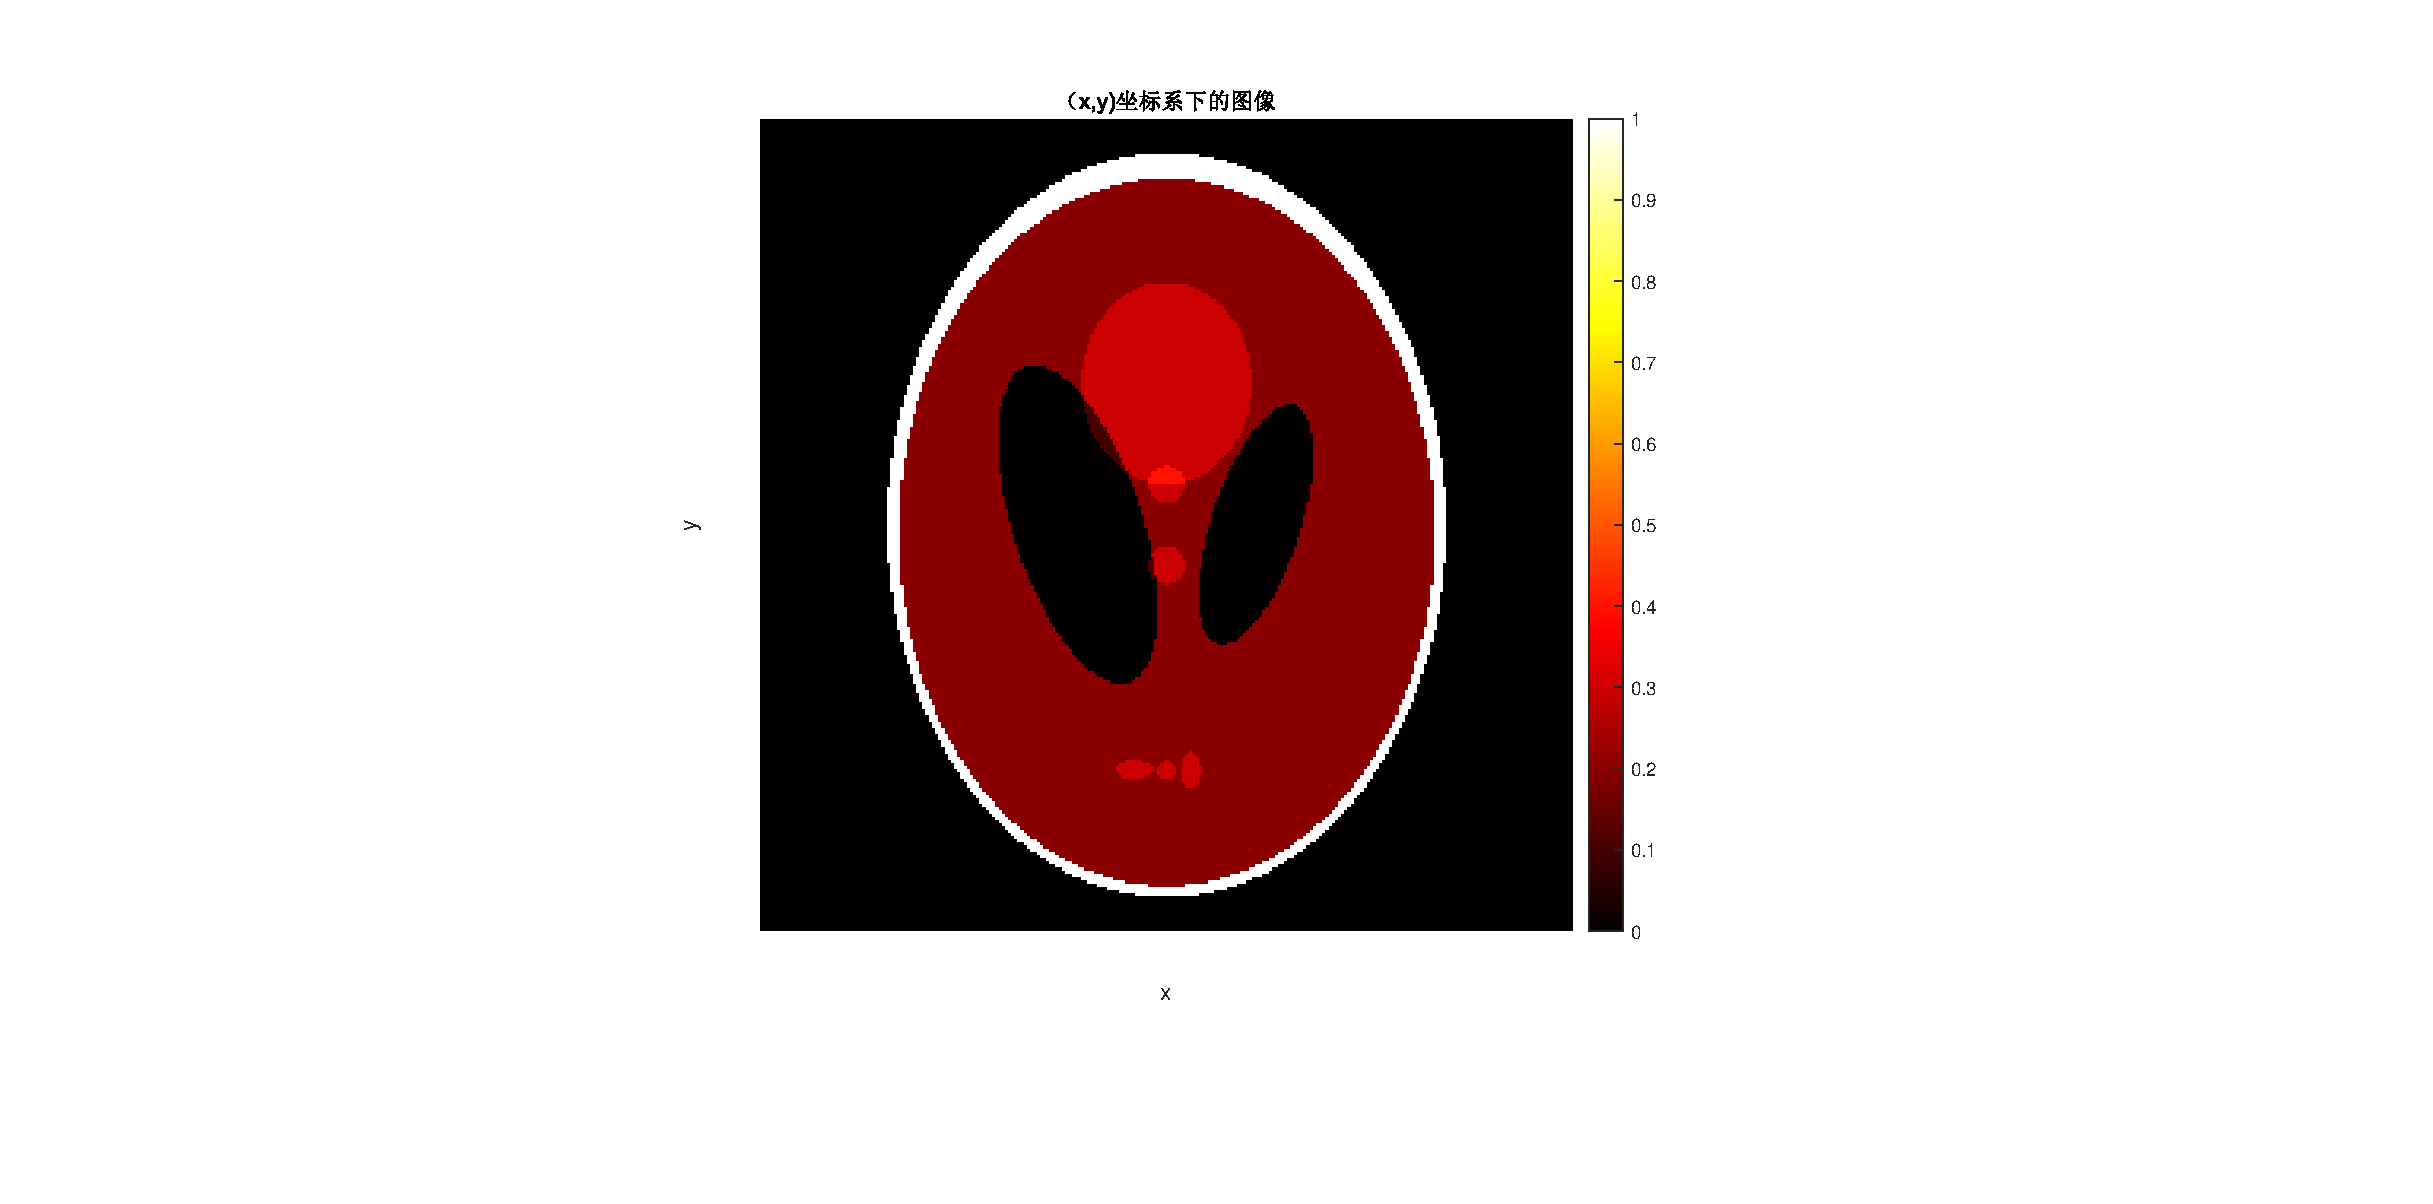
\includegraphics[width=90mm]{Radon_Origin.eps}
			    \caption{$Radon$变换前原图像}
			    \label{fig:a}
			  \end{minipage}%
			  \begin{minipage}[b]{0.5\linewidth}
			    \centering
			    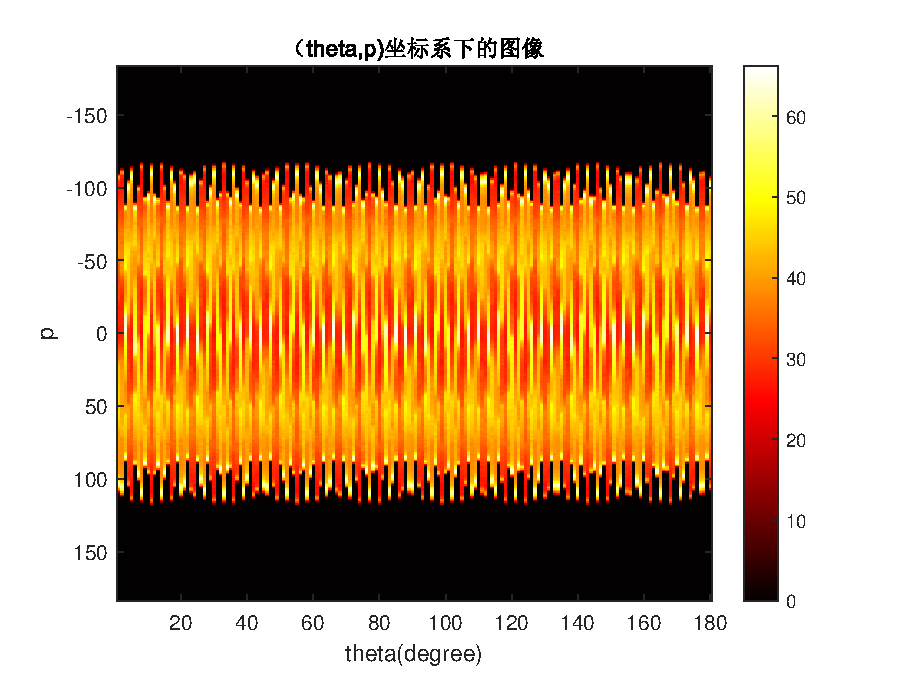
\includegraphics[width=60mm]{Radon_full_dose.eps}
			    \caption{$Radon$变换后图像}
			    \label{fig:b}
			  \end{minipage}
			\end{figure}
	
	\section{滤波反投影($FBP$)算法描述}
		随着$CT$技术的发展,重建算法也变得多种多样,各有各的有特点。本文介绍目前应用最广泛的重建算法——滤波反投影算法($FBP$)作为模型的基础算法。$FBP$算法是在傅立叶变换理论基础之上的一种空域处理技术。它的特点是在反投影前将每一个采集投影角度下的投影进行卷积处理,从而改善点扩散函数引起的形状伪影,重建的图像质量较好。

		\subsection{$FBP$算法原理}
			\subsubsection{中心切片定理}
				我们先来回顾一个经典定理——中心切片定理。即:
		
				密度函数在某一方向上的投影函数的一维傅立叶变换函数是原密度函数的二维傅立叶变换函数在平面上沿同一方向且过原点的直线上值。如figure\ref{中心切片定理}所示。
				\begin{figure}[ht!]
					\centering
					\includegraphics[width=150mm]{中心切片定理.png}
					\caption{中心切片定理示意图 \label{中心切片定理}}
				\end{figure}
					
				figure\ref{中心切片定理}可以清晰的描述傅立叶中心切片定理的过程:对投影的一维傅立叶变换等效于对原图像进行二维的傅立叶变换。
		
				傅立叶切片定理的意义在于,通过投影上执行傅立叶变换,可以从每个投影中得到二维傅立叶变换。从而投影图像重建的问题,可以按以下方法进行求解:采集不同时间下足够多的投影(一般为180次采集),求解各个投影的一维傅立叶变换,将上述切片汇集成图像的二维傅立叶变换,再利用傅立叶反变换求得重建图像。

			\subsubsection{滤波反投影算法原理分析}
				1、在不同的角度下取得足够多的投影数据($Radon$变换)

				2、将这些投影数据做一维的$Fourier$变换,那么变换后的这些数据将充满整个$(u,v)$平面。(许多过原点成不同夹角的直线)

				3、也就是说,$F(u,v)$的全部值都为已知,那么我们将其做一次二维的$Fourier$逆变换就可以得到原始的衰减系数函数$f(x,y)$。即
				
				\begin{equation}
					\quad f(x, y)=\iint_{-\infty}^{+\infty} F(u, v) \exp [j 2 \pi(u x+v y)] d u d v
				\end{equation}

				作坐标变换, 令: 
				\begin{equation}
					u=\rho \cos \theta \quad v=\rho \sin \theta
				\end{equation}

				可得出:
				\begin{equation}
					\begin{aligned}
					&f(x, y)=\int_{0}^{\pi+\infty} \int_{-\infty}^{+\infty} F(\rho, \theta)|\rho| e^{j 2 \pi \rho(x \cos \theta+y \sin \theta)} d \rho d \theta \\
					&=\int_{0}^{\pi} d \theta \int_{-\infty}^{+\infty}\left[F(\rho, \theta)|\rho| e^{j 2 \pi \rho R} d \rho\right] \delta(x \cos \theta+y \sin \theta-R) \mathrm{dR} \\
					&=\int_{0}^{\pi} d \theta \int_{-\infty}^{+\infty} g_{\theta}^{\prime}(\mathrm{R}) \delta(x \cos \theta+y \sin \theta-R) \mathrm{dR} \\				
					\end{aligned}
				\end{equation}

				\begin{equation}
					g_{\theta}^{\prime}(\mathrm{R})=\int_{-\infty}^{+\infty} F(\rho, \theta)|\rho| e^{j 2 \pi \rho R} d \rho
				\end{equation}

				表示对投影函数的$Fourier$变换进行滤波变换,其中 $|\rho|$ 是滤波函数。
	
				由傅立叶变换性质可知.频域中的滤波运算可等效地在空域中用卷积运算来完成。所以
				\begin{equation}
					\int_{0}^{\pi} d \theta \int_{-\infty}^{+\infty}[g_{\theta}(\mathrm{R})*h(\mathrm{R})]\delta(x \cos \theta+y \sin \theta-R) \mathrm{dR}
				\end{equation}

				式中$h(\mathrm{R})$为滤波函数的空域形式

			\subsubsection{滤波反投影重建算法过程}
				投影重建的过程是,先把投影由线阵探测器上获得的投影数据进行一次一维傅立叶变换,再与滤波器函数进行卷积运算,得到各个方向卷积滤波后的投影数据;然后把它们沿各个方向进行反投影,即按其原路径平均分配到每一矩阵单元上,进行重叠后得到每一矩阵单元的$CT$值;再经过适当处理后得到被扫描物体的断层图像。
				
				算法步骤如下:

				1. 将原始投影进行一次一维傅立叶变换

				2. 设计合适的滤波器,在$φ_{i}$的角度下将得到原始投影$p(x_{r},φ_{i})$进行卷积滤波,得到滤波后的投影。

				3. 将滤波后的投影进行反投影,得到满足$x_{r}=r \cos ((\theta⁡ - φ_{i}))$方向上的原图像的密度。

				4. 将所有反投影进行叠加,得到重建后的投影。

		\subsection{滤波函数}
			滤波函数的选取是滤波反投影法的关键问题。滤波反投影算法结果的好坏很大程度上取决于滤波函数的选择。下面介绍两种滤波函数,$R-L$滤波函数和$S-L$滤波函数。 

			(1)$R-L$滤波函数

				由于在频域中用矩形函数截断了滤波函数,在相应的空域中造成振荡响应 ,重建的图像质量往往不够满意。对应的频域形式为:
				\begin{equation}	
					H(\rho)=|\rho| \operatorname{rect}\left(\frac{\rho}{2 \rho_{0}}\right)
				\end{equation}

				理想的滤波函数$|\rho|$它是在高频的权重很大,低频的权重很小,所以高频噪声就会很大,所以我们才要对其进行修正。

			(2)$S-L$滤波函数

	      与$R-L$滤波函数不同的是,$S-L$滤波函数它的关键是把频域的陡峭截止改成缓慢截止。

	      用$S-L$滤波函数重建的图像中振荡相应较小,对含噪声的数据重建出来的图像质量也较$R-L$滤波函数重建的图像质量要好。但是,$S-L$滤波函数重建的图像在高频响应方面不如$R-L$滤波函数好,这是因为$S-L$滤波函数在高频段偏离了理想的滤波函数。对应的频域形式为:如figure\ref{滤波函数}所示
			\begin{equation}
				H_{S-L}(\rho)=|\rho| \sin c\left(\frac{\rho}{2 \rho_{0}}\right) \operatorname{rect}\left(\frac{\rho}{2 \rho_{0}}\right)
			\end{equation}
			\begin{figure}[ht!]
				\centering
				\includegraphics[width=120mm]{滤波函数.png}
				\caption{滤波函数($R-L,S-L$) \label{滤波函数}}
			\end{figure}
			
		\subsection{实验结果及其分析}
			\subsubsection{滤波器(滤波函数)和内插函数的选取}
				由于直接使用反投影算法会存在两个对实验结果影响很不好的因素:

					1.不准确的数据重建图像就会产生各种伪影。
					
					2.投影的数据是天然离散的,处理不当的话会产生很大的误差。
		
				常见的滤波器有$R-S$滤波函数和$S-L$滤波函数。$R-L$滤波函数滤波计算简单,避免了大量的正弦、余弦计算,得到的采样序列分是分段现行的,并没有明显的降低图像质量,所以重建图像轮廓清楚,空间分辨率高。

				常见的插值方法有最近邻插值和双线插值,最近邻插值即将离散点中间的缺失值用离它最近的整数处的投影值来替代。

			\subsubsection{$FBP$算法案例实现}
				我们根据上面的步骤进行代码撰写,然后根据我们撰写的代码进行实验(见附录B)。

				我们先使用$Matlab$上自带的$Shepp\ Logan$模型,生成一个原图像。如figure \ref{原图像}所示
			\begin{figure}
			  \begin{minipage}[ht!]{0.5\linewidth}
			    \centering
			    
\includegraphics[width=60mm]{origin.eps}
					\caption{原图像 \label{原图像}}
			  \end{minipage}%
			  \begin{minipage}[ht!]{0.5\linewidth}
			    \centering
					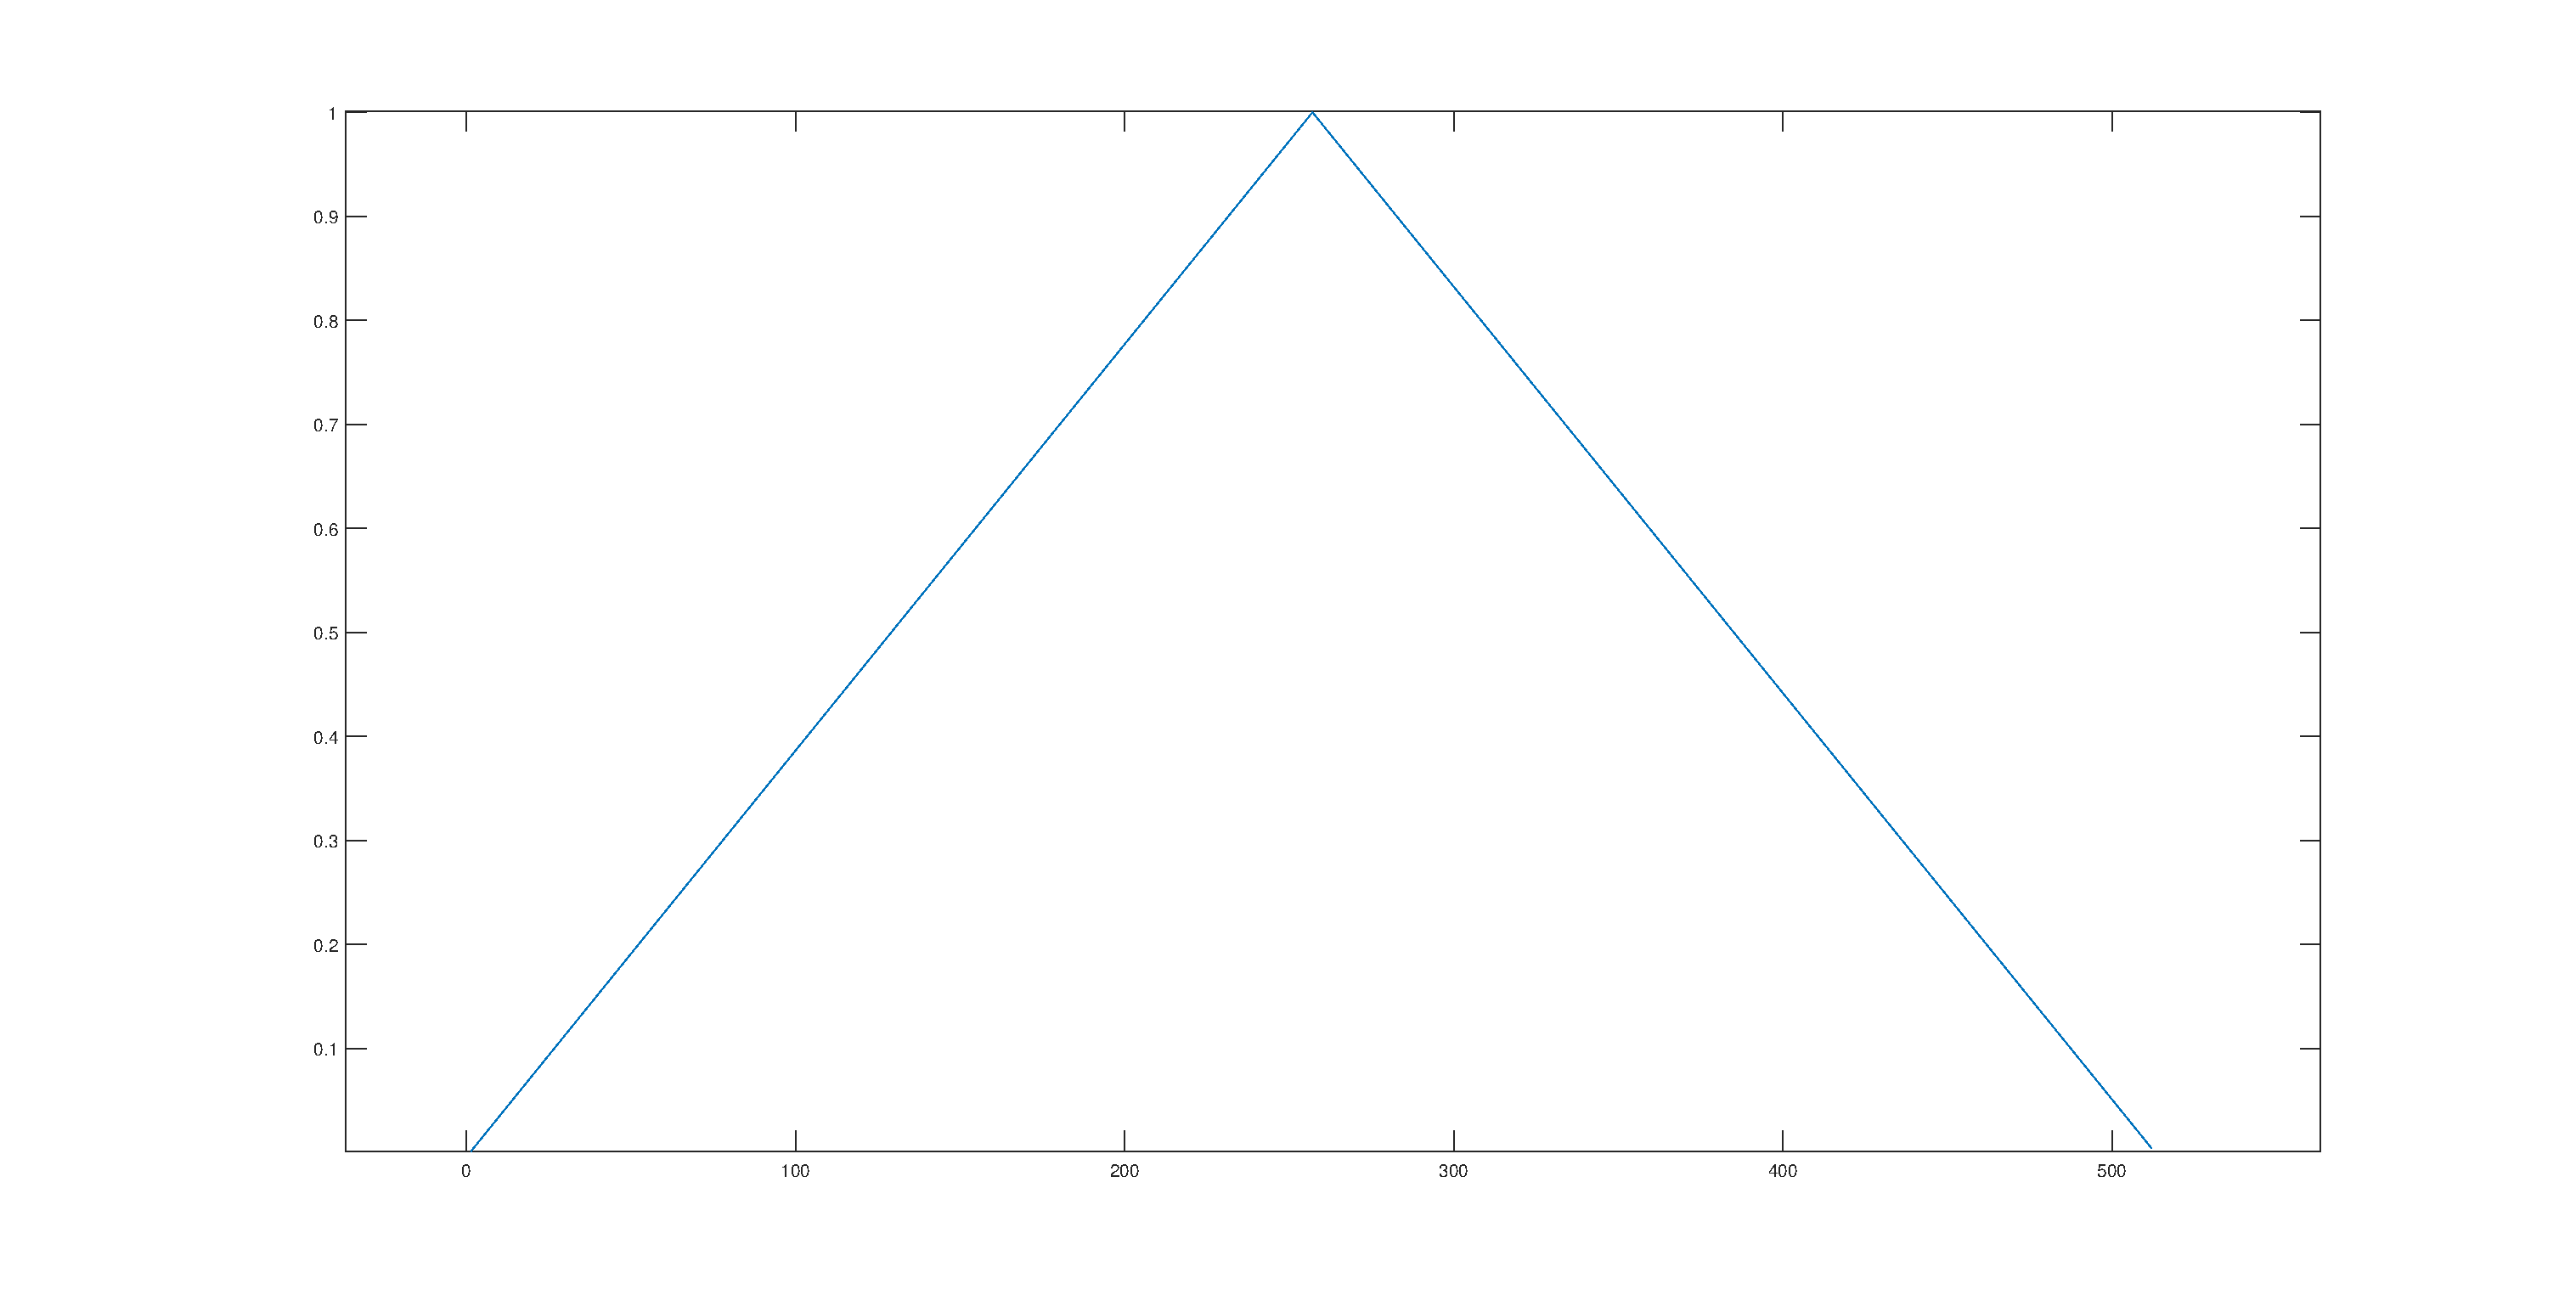
\includegraphics[width=60mm]{fttplot.eps}
					\caption{窗函数 \label{窗函数}}
			  \end{minipage}
			\end{figure}
				
				然后对原图像进行快速傅里叶变换($FFT$)。如figure \ref{fft}所示。
			\begin{figure}
			  \begin{minipage}[ht!]{0.5\linewidth}
			    \centering
					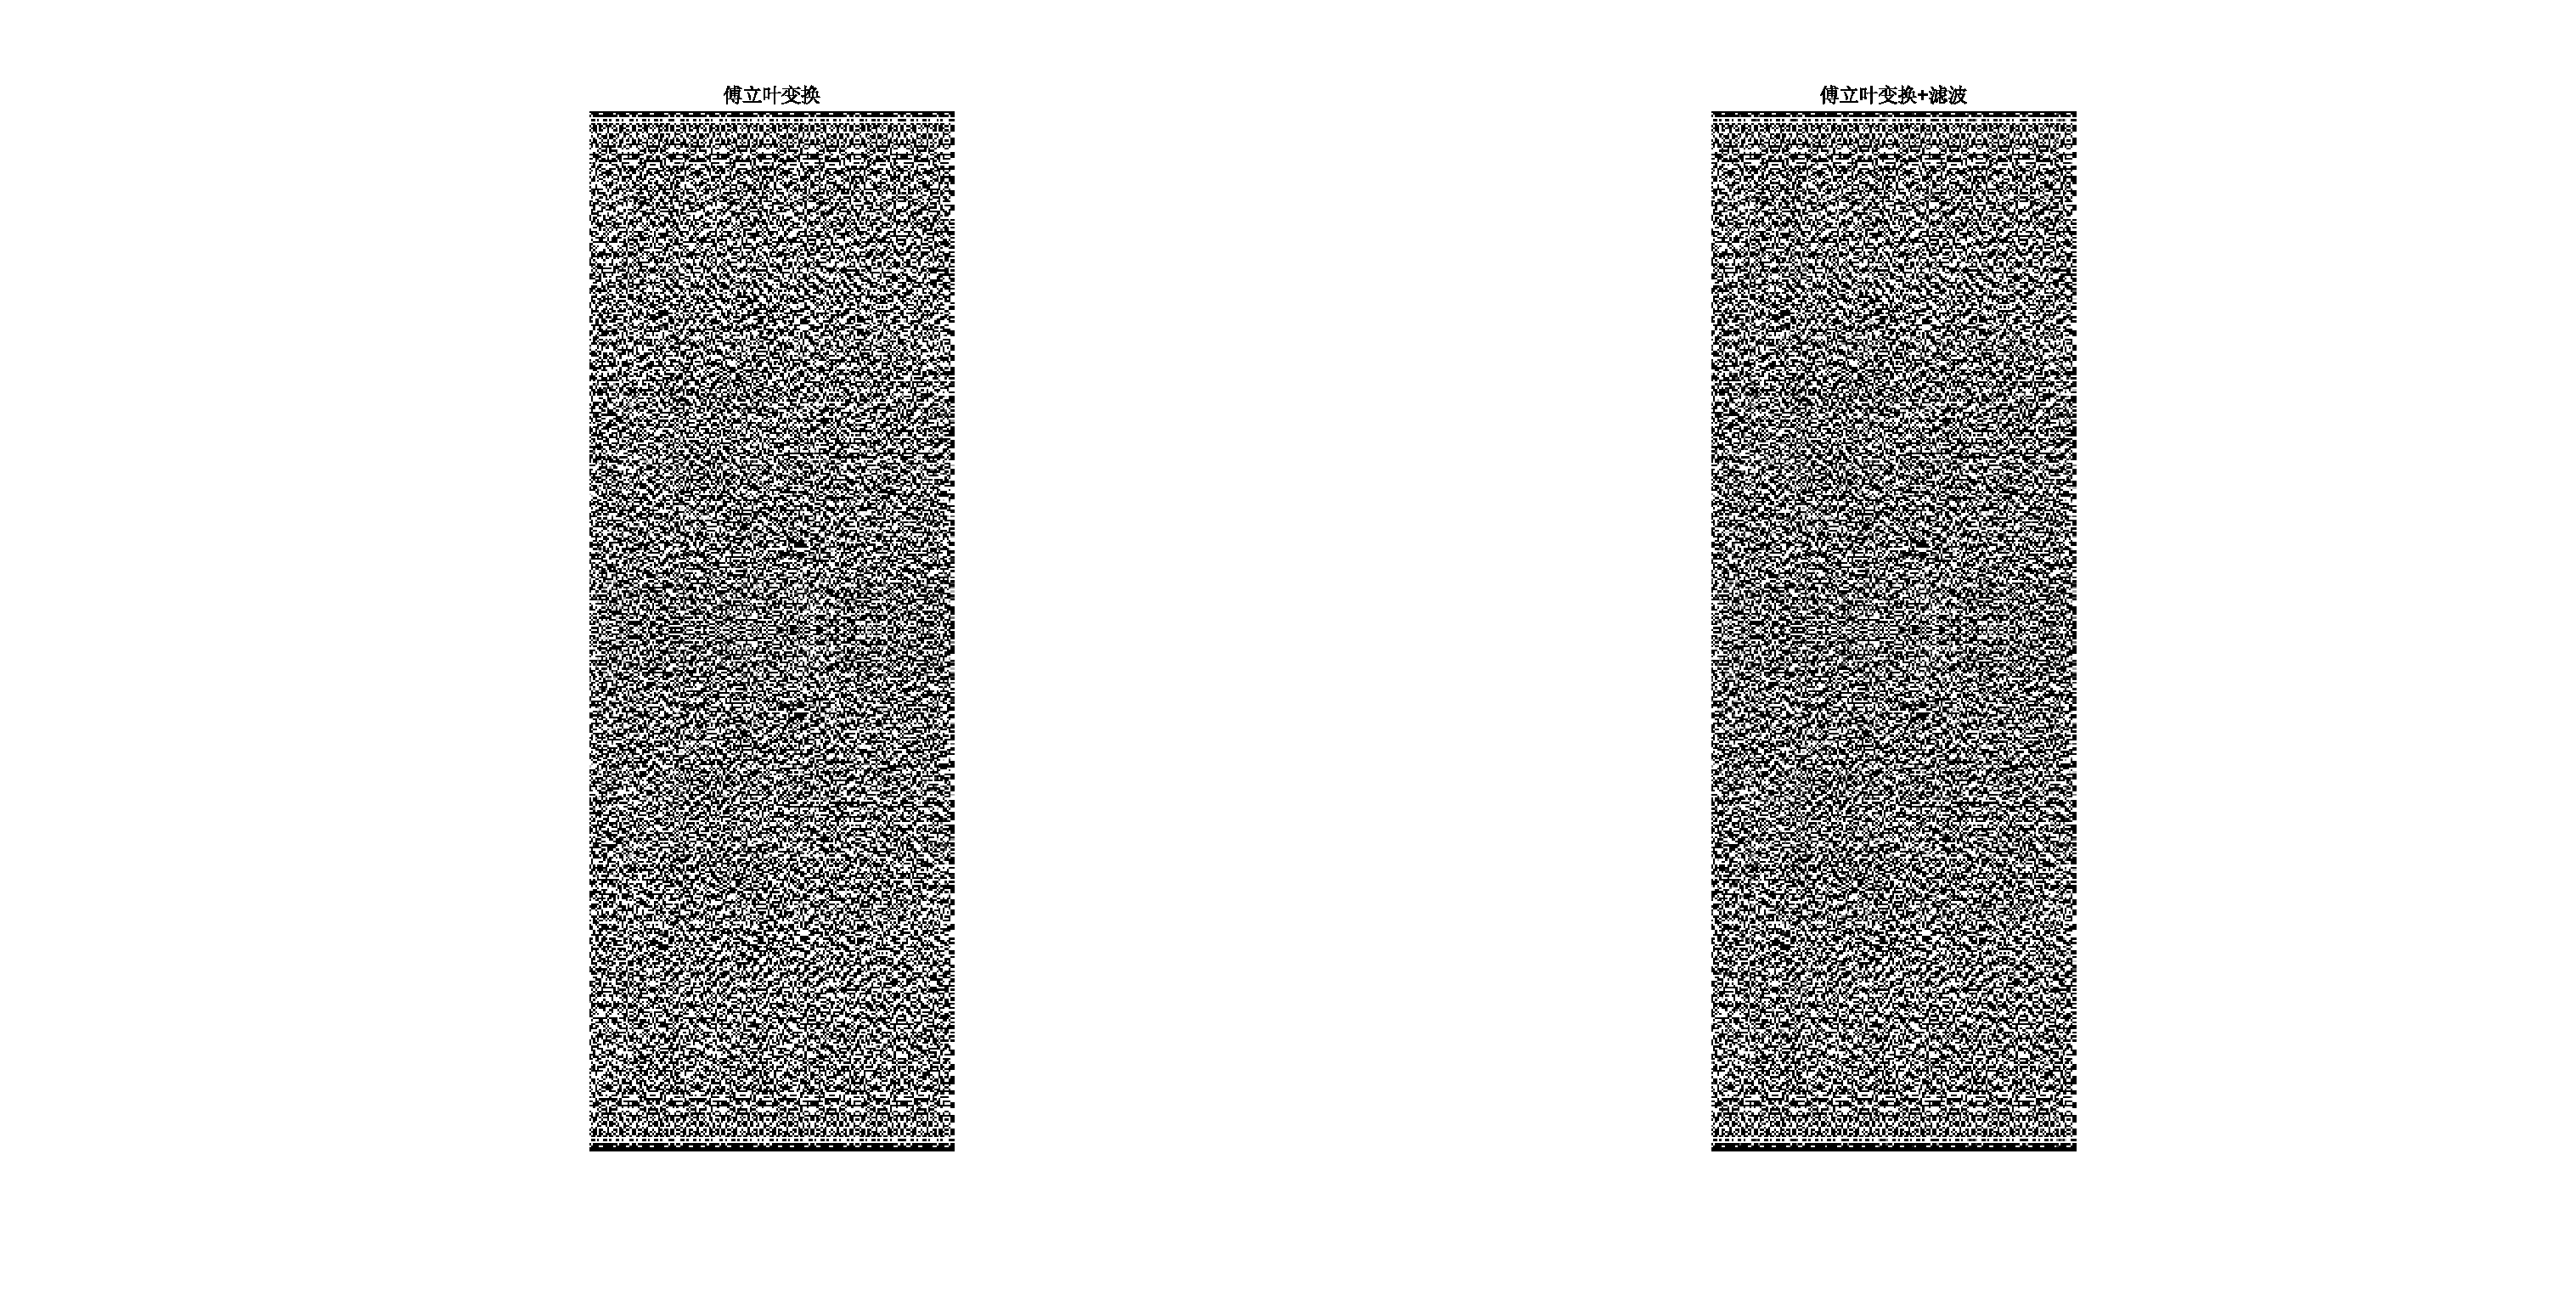
\includegraphics[width=60mm]{fourier_transform.eps}
					\caption{快速傅里叶变换图像 \label{fft}}
			  \end{minipage}%
			  \begin{minipage}[ht!]{0.5\linewidth}
			    \centering
					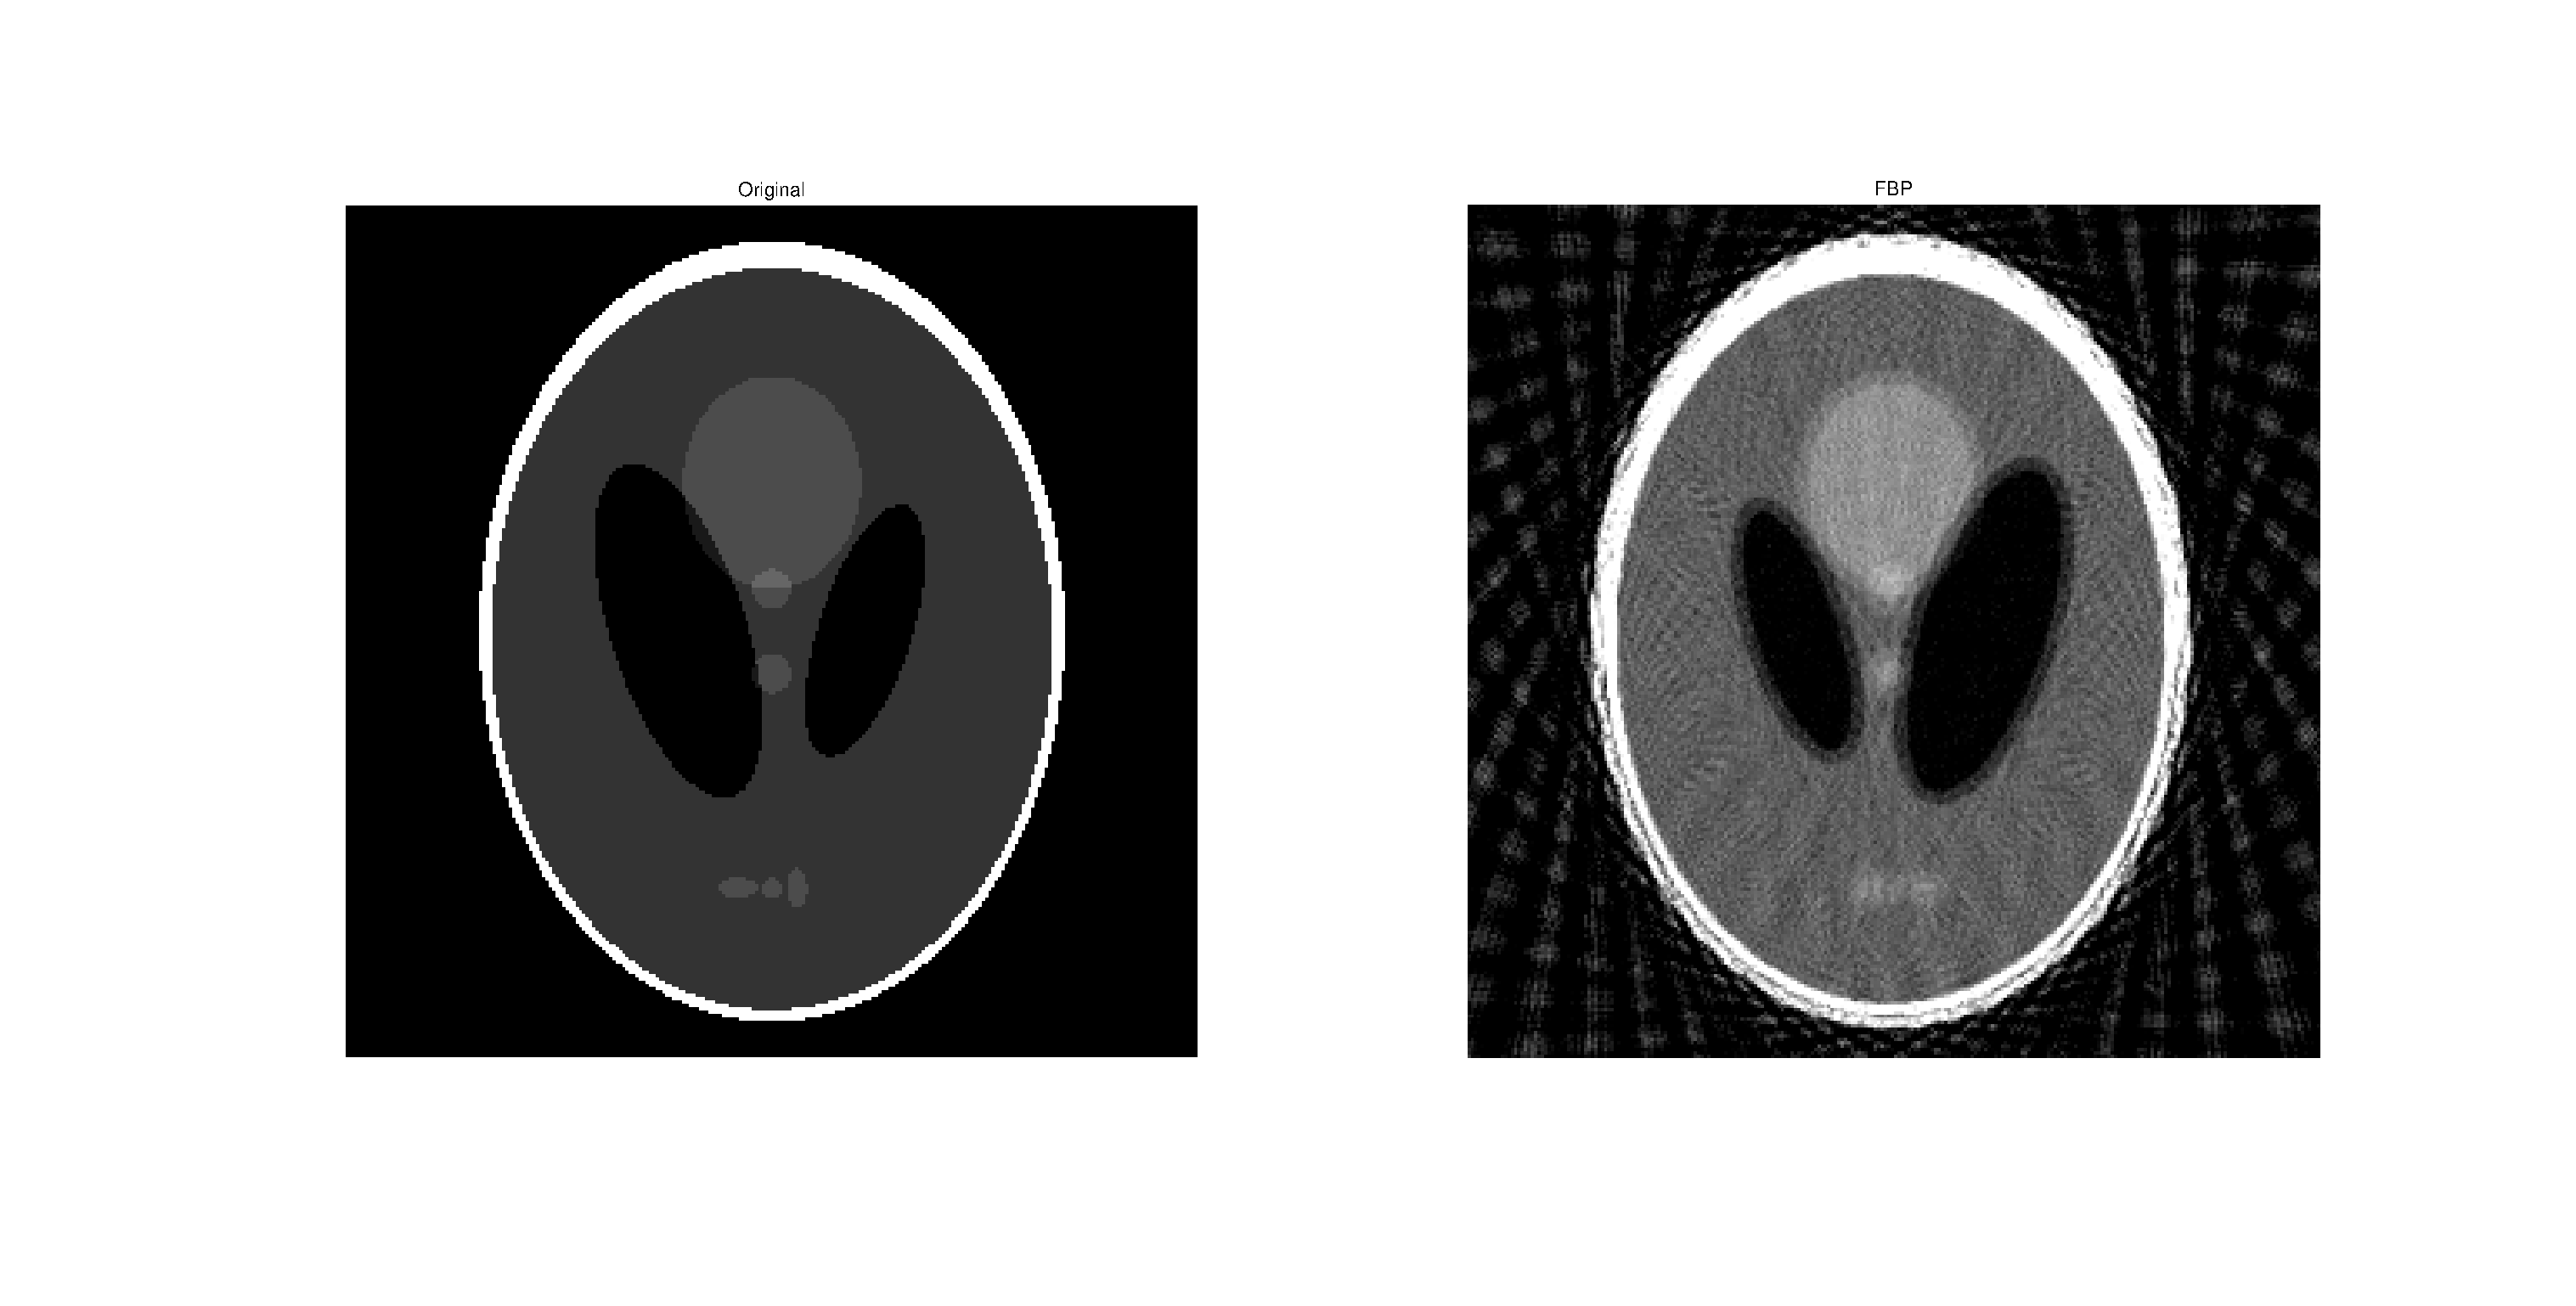
\includegraphics[width=60mm]{fbp256.eps}
					\caption{原图像与$FBP$算法重建图像 \label{fbp对比图像}}
			  \end{minipage}
			\end{figure}

				再对所得数据进行滤波操作。其中figure\ref{窗函数}为算法使用的窗函数即$R-L$滤波函数,用于对投影做快速傅里叶变换后进行滤波操作。
				
				最后我们将得到的数据再进行逆快速傅里叶变换并进行反投影,得到重建图像,将变换后的图像和原图像进行比照。如figure \ref{fbp对比图像}所示。发现效果良好。

	\section{变换法缺点(投影数据的多少对重建效果的影响)}
		
		在$Matlab$图像处理工具箱中,有$phantom$函数,可以用来创建头部的剖视图,首先创建一个头部的256×256剖视图,然后分别计算3组不同的$Radon$变换,第一组采用30个投影,第二组采用90个投影,第三组采用180个投影,用以比较采用不同组数的投影参数重建的图像与原始图像的差别。 如figure\ref{对比}所示。
		\begin{figure}[ht!]
				\centering
				\includegraphics[width=150mm]{对比.png}
				\caption{不同数量的投影数据重建图像对比图 \label{对比}}
		\end{figure}

		所以看似完美的滤波反投影算法有个致命的问题(直接傅里叶变换等变换法均存在这类问题),就是如果投影数据是不完全的,是否还能重建出完整的图像。这个问题使用变换法很难解决。于是在$Gordon$、$Bender$和$Herman$等人的努力下,将求解大型线性方程组的解的方法引入到图像重建领域里来。成功的解决了不完全数据图像重建的问题。

	\section{代数重建($ART$)算法描述}
		我们先来回到问题的起点——图像重建。前面已经明确,图像重建方法一般有两种方法。变换法在前面已经叙述,在迭代重建法中有多种不同的类型。其中研究和应用最为广泛的有:代数重建法($ART$)、 同时联合迭代重建法($SART$)和最大熵值法($ME$)

		滤波反投影算法要求投影数据必须是完全的,分布必须均匀。具体地说就是采集数据时应覆盖物体的全部区域,相邻射线间均为$d$。然而实际应用中,有时无法采集大量的投影数据。例如做$CT$时,为了避免心脏器官受辐射过久,采集到的数据不是完全的,滤波反投影方法就不能很好的重建图像。

		而代数重建算法($ART$)是将图像重建问题转化为解线性方程组,丢失投影数据可以看作是缺少方程,因而适合于不完全投影数据的重建,并能利用某些先验知识提高重建图像质量。

		\subsection{原理}
			英文名称为$Algebraic reconstruction technique$:即代数重建算法。代数重建技术($ART$)是一种用于计算机层析成像的迭代重建技术。它从一系列的角度投影(正弦图)中重建一幅图像。$Gordon$、$Bender$和$Herman$首次证明了它在图像重建中的应用。而这种方法被称为数值线性代数中的$Kaczmarz$方法。相对于其他重建方法(如滤波反投影),$ART$的一个优点是,将先验知识(已知的约束条件)纳入重建过程是相对容易的。该算法的实质是用迭代法求解线性方程组的解,我们将该方程表示为:
			\begin{equation}
				Ax=b
			\end{equation}

			代数重建算法的本质其实就是通过迭代的方法近似求解上述方程组,以达到图像重建的目的。
			\subsubsection{示例}
			如下列图像重建问题:见图figure\ref{ART示例}
			\begin{figure}[ht!]
				\centering
				\includegraphics[width=120mm]{ART示例.jpg}
				\caption{$ART$示例 \label{ART示例}}
			\end{figure}

			其图像重建问题对应于解下列线性方程组:
			\begin{equation}
				\left\{\begin{aligned}
				x_{1}+x_{2}+x_{3} &=p_{1} \\
				x_{4}+x_{5}+x_{6} &=p_{2} \\
				x_{7}+x_{8}+x_{9} &=p_{3} \\
				x_{3}+x_{6}+x_{9} &=p_{4} \\
				x_{2}+x_{5}+x_{8} &=p_{5} \\
				x_{1}+x_{4}+x_{7} &=p_{6} \\
				2(\sqrt{2}-1) x_{4}+(2-\sqrt{2}) x_{7}+2(\sqrt{2}-1) x_{8}&=p_{7} \\
				\sqrt{2} x_{1}+\sqrt{2} x_{5}+\sqrt{2} x_{9}&=p_{8} \\
				2(\sqrt{2}-1) x_{2}+(2-\sqrt{2}) x_{3}+2(\sqrt{2}-1) x_{6}&=p_{9}
				\end{aligned}\right.
			\end{equation}
		
			这个方程组转化为矩阵的形式即为(1)式。
		
			其中, $X=\left[x_{1}, x_{2}, \ldots, x_{9}\right]^{T}, \quad b=\left[b_{1}, b_{2}, \ldots, b_{9}\right]^{T}$ 
		
			迭代算法的思想使将$AX=b$变换为以下迭代形式
			\begin{equation}
				X^{(i+1)}=G X^{(i)}+b
			\end{equation}
			
			通过不同的变换方式变成迭代格式, 就产生了不同的的迭代算法。经典方法是$Gorden\ R.$等提出的代数重建法($ART$),此外还有联合代数重建方法($SART$)和乘型代数重建方法($Multiplicative ATR ,MATR$)。

			\subsubsection{基本思想}

			先给定一个初始图像 $\mathrm{x}^{(0)}$ 求一次近似图像 $\mathrm{x}^{(1)}$, 再据 $\mathrm{x}^{(1)}$ 求二次近似图像 $\mathrm{x}^{(2)}$,

			如此继续, 直至满足预定条件而后止。在根据 $\mathrm{x}^{(\mathrm{k})}$ 求 $\mathrm{x}^{(\mathrm{k}+1)}$ 时需加一校正值 $\Delta \mathrm{x}^{(k)}$ 。 $A R T$ 满足线性不等式 $A x \leq b$

			而对于图像重建这一具体的情况, 我们可以将上式写成 $r_{i}^{T} x \leq b_{i} \quad i=1,2, \cdots, I$

			而上式的解, 也即$ART$的迭代公式如下:

			$x^{(0)}$, 任意;
	
			$x^{(k+1)}=\left\{\begin{array}{c}x^{(k)} \quad r_{i k}^{T} x^{(k)} \leq b_{i k} ; \\ x^{(k)}+\lambda^{(k)} \frac{b_{i k}-r_{i k}^{T} x^{(k)}}{\left\|r_{i k}\right\|^{2}} r_{i k} \quad \text { 其他 }\end{array}\right.$

			其中 $i_{k}=k(\bmod I)+1$

		\subsection{几何意义}
			
			\subsubsection{可视化}
				为了深入理解算法的几何意义,我们讲算法求解的过程可视化,画出方程的解的轨迹,如图所示。(代码见附录C)
				\begin{figure}[ht!]
				\centering
				\includegraphics[width=120mm]{VisualizationART_0.png}
				\caption{算法求解轨迹 \label{算法求解轨迹图}}
				\end{figure}

			\subsubsection{几何意义}
				对迭代公式: 
				\begin{equation}
					x^{(1)}=x^{(0)}+\frac{p_{1}-r_{1}^{T} x^{(0)}}{\left\|r_{1}\right\|^{2}} r_{1}
				\end{equation}

				校正项 $\frac{p_{1}-r_{1}^{T} x^{(0)}}{\left\|r_{1}\right\|^{2}} r_{1}$,\;
				改写成 $\frac{p_{1}-r_{1}^{T} x^{(0)}}{\left\|r_{1}\right\|} \cdot \frac{r_{1}}{\left\|r_{1}\right\|}$
				
				其中,$\left\|r_{i}\right\|$代表 $x^{(0)}$ 到 $H$ 的距离。$\frac{r_{1}}{\left\|r_{i}\right\|}$ 是 $r_{i}$ 的单位矢量, 即 $H$ 的单位法向量。、

				所以上式既描述了校正值的大小,又指出了他的方向,具体来说就是,如果$p_{1}-r_{1}^{T} x^{(0)}<0$即$p_{1}<r_{1}^{T} x^{(0)}$,那么校正值就会指向$r_{1}$的反方向,企图缩短$x^{(0)}$到$x$(真实值)的欧式距离。
				\begin{figure}[ht!]
				\centering
				\includegraphics[width=120mm]{ART_geo.png}
				\caption{几何意义示意图 \label{几何意义示意图}}
				\end{figure}

			\subsubsection{物理意义}
				
				校正项 $\frac{p_{1}-r_{1}^{T} x^{(0)}}{\left\|r_{1}\right\|^{2}} r_{1}$

				$p_{1}$ 为测得的射线1的射线投影, 称为真射线和。

				$r_{1}^{T} x^{(0)}$表示图像矢量为 $x^{(0)}$ 时, 射线1的伪射线和 $\mathrm{p}_{1}^{(0)}$ 

				$p_{1}-r_{1}^{T} x^{(0)}=\Delta p_{1}$ 称为校正投影。经过加权 $\frac{1}{\left\|r_{1}\right\|^{2}}$ 后形成 $\frac{\Delta p_{1}}{\left\|r_{1}\right\|^{2}}$, 沿射线 1反投影于该射线经过的像素,去校正这些像素值。 

				例如像素 1 受到的反投影值为 $\frac{\Delta p_{1}}{\left\|r_{1}\right\|^{2}} r_{11}=\Delta x_{1}$

				像素2受到的反投影值为 $\frac{\Delta p_{1}}{\left\|r_{1}\right\|^{2}} r_{12}=\Delta x_{2}$

				不在射线 1 上的像素 $j$ ,其 $r_{1 j}=0$, 自然也就不受该 $\Delta p_{1}$ 的影响。

			
		\subsection{实验结果及其分析}

			\subsubsection{计算结果}
				步骤:
	
    			$Algebraic Reconstruction Technique$ ($ART$) 代数重建算法其实就是解一个方程,射束组成一个一维数组,记为 $\left[p_{1}, p_{2}, \ldots, p_{m}\right]$,其中 $m$ 为穿过物体的x射线的条数,它等于投影角度与每个投影角度上射束的条目的乘积,则 有方程组:
		    \begin{equation}
			     \left\{\begin{array}{l}
			     \omega_{11} f_{1}+\omega_{12} f_{2}+\ldots+\omega_{1 N} f_{N}=p_{1} \\
			     \omega_{21} f_{1}+\omega_{22} f_{2}+\ldots+\omega_{2 N} f_{N}=p_{2} \\
			     \cdots \\
			     \omega_{m 1} f_{1}+\omega_{m 2} f_{2}+\ldots+\omega_{m N} f_{N}=p_{m}
			     \end{array}\right.
		    \end{equation}

    			一共$N$个末知数 $\left(f_{1}, f_{2}, \ldots, f_{N}\right)$ , $M$ 个方程,其中的 $\omega_{i j}$ 就是前面介绍的投影矩阵的元素。我们只要进行以下形式的迭代:
		    \begin{equation}
			     f_{j}^{k+1}=f_{j}^{k}+\lambda \frac{p_{i}-\sum_{n=1}^{N} w_{i n} f_{n}^{k}}{\sum_{n=1}^{N} \omega_{i n}^{2}} \omega_{i j}, \quad j=1,2, \ldots, N
		    \end{equation}
    			
				进行一次迭代就是一次投影和反投影操作,我们可以进行多次迭代,直到结果收敛(代码见附录C)。计算结果如figure\ref{ART算法结果}和figure\ref{ART算法结果对比}所示。
				\begin{figure}[ht!]
				\centering
				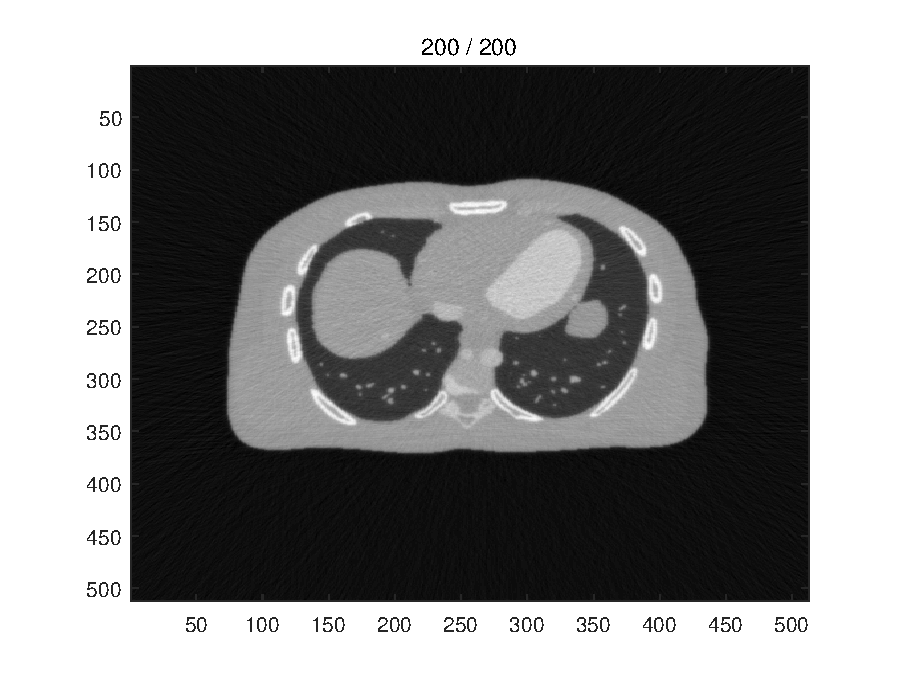
\includegraphics[width=120mm]{ART_result2.eps}
				\caption{$ART$算法结果 \label{ART算法结果}}
		\end{figure}

				\begin{figure}[ht!]
				\centering
				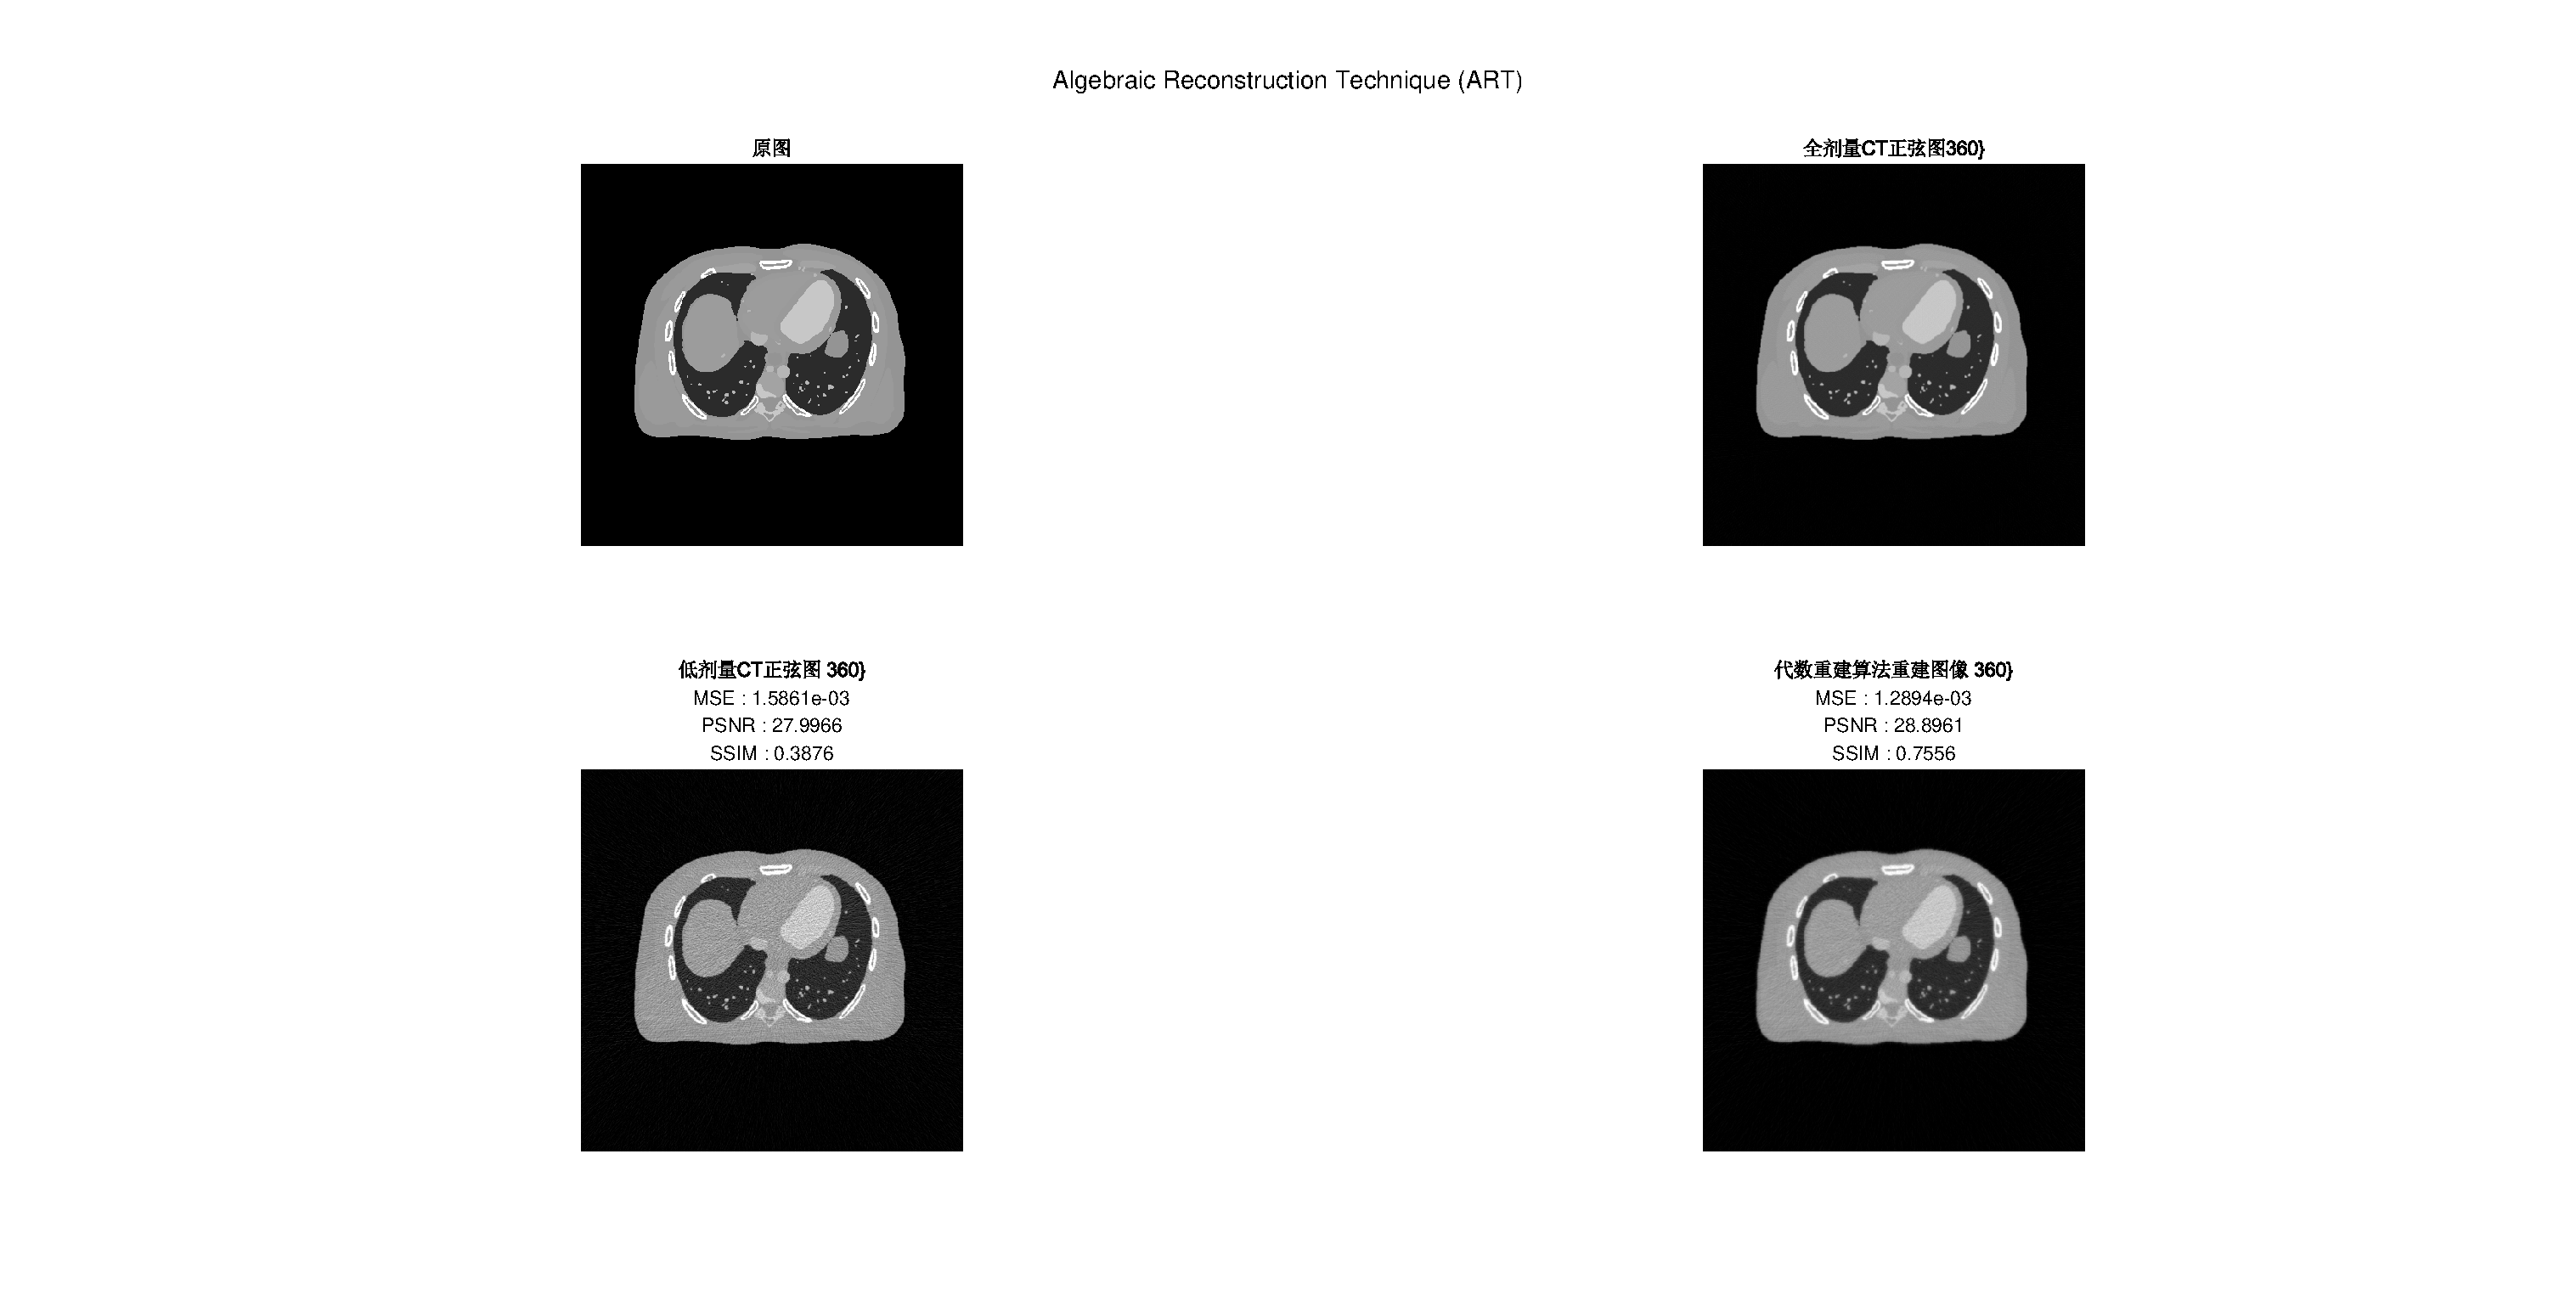
\includegraphics[width=150mm]{ART_result.eps}
				\caption{$ART$算法结果对比 \label{ART算法结果对比}}
		\end{figure}
	\newpage
	\section{算法比较}
		两种方法各有优劣,适合于不同的场景。
	\section{总结}
		本文主要介绍了图像重建方法里面的滤波反投影方法和代数重建方法的理论,并且带入$Shepp\ Logan$进行图像重建。理清了图像重建领域的发展历程,明确了图像重建由变换法到级数展开法的发展变化。
	
	\section*{Acknowledgments}
	 感谢渠刚荣老师一学期的陪伴,学习的很多知识,实现了很多算法,大学以来最开阔数学视野的课程大概就是这门课程了。同时通过这门课程我也对图像重建这个领域产生了浓厚的兴趣。在大作业的撰写过程中,编写$LaTeX$的能力飞速提升。总之收获良多,感恩满满。
	%\newpage
	%\begin{thebibliography}{100}%此处数字为最多可添加的参考文献数量
	%	\bibitem{article1}ART%title author journal data pages
	%	\bibitem{book1}This is reference.%title author publish date
	%\end{thebibliography}
	%\end{multicols}
	\newpage
	\begin{appendices}
		\section{$Radon$变换$Matlab$代码}
			\begin{lstlisting}
function [P,r] = radon_0(I,theta,n)
%Radon变换函数实现代码
    validateattributes(I,{'numeric','logical'},{'2d','nonsparse'},mfilename,'I',1);
    if(nargin < 2)
        theta = 0:179;
    else
        validateattributes(theta,{'double'},{'real','nonsparse','vector'},mfilename,'THETA',2);
    end
    [P,r] = images.internal.builtins.radonc(double(I),theta);

if (nargin == 3)
    validateattributes(n,{'double'},{'real','positive','scalar','integer'},mfilename,'n',3);
    if size(P,1) ~= n
        new_r = linspace(min(r), max(r), n)';
        P = interp1(r(:), P, new_r(:), '*linear');
        P = P * length(r) / length(new_r); 
        r = new_r;
    end
end
			\end{lstlisting}

			\begin{lstlisting}	%正文插入代码

function RadonTest()
%% Radon Transform此代码用来可视化
M = 256; %指定原图片像素
P = phantom(M); % 创建一个 shepp-logan 模型,原图像
figure(1),imshow(P);%画原图
title('(x,y)坐标系下的图像'); 
xlabel('x'); 
ylabel('y'); 
colormap(hot);  
colorbar;

theta=1:180; %角度
[R,x]=radon_0(P,theta*180/pi);%利用自己写的radon_0函数进行Radon变换获得不同方向上的投影
figure(2),imagesc(theta,x,R);%画变换之后的图 
title('(theta,p)坐标系下的图像'); 
xlabel('theta(degree)'); 
ylabel('p'); 
colormap(hot);  
colorbar;

end
    	\end{lstlisting}
		\newpage
		\section{滤波反投影($FBP$)算法$Matlab$代码}
    	\begin{lstlisting}
%% 创建图像及投影
M=256;
P = phantom(M); % 创建一个 shepp-logan 模型,原图像
theta=1:180; %角度
[R,xp] = radon(P,(theta*180)/pi);%利用radon变换获得不同方向上的投影
xp_offset = abs(min(xp) + 1);
%% 傅立叶变换
size(R,1);%367
width = 2^nextpow2(size(R,1)); %傅立叶变换的宽度
proj_fft = fft(R, width);
filter = 2*[0:(width/2-1), width/2:-1:1]'/width;
figure(1),plot(filter)
proj_filtered = zeros(width,180);
figure(2),subplot(1,2,1),imshow(proj_fft),title('傅立叶变换');
subplot(1,2,2),imshow(proj_filtered),title('傅立叶变换+滤波')
for i = 1:180
    proj_filtered(:,i) = proj_fft(:,i).*filter;
end
%% 逆傅里叶变换并反投影
proj_ifft = real(ifft(proj_filtered)); 
fbp = zeros(M); 
for i = 1:180
    rad = theta(i);
    for x = (-M/2+1):M/2
        for y = (-M/2+1):M/2
            t = round(x*cos(rad+pi/2)-y*sin(rad+pi/2)+xp_offset);
            fbp(x+M/2,y+M/2)=fbp(x+M/2,y+M/2)+proj_ifft(t ,i);
        end
    end
end
fbp =(fbp*pi)/180;%256x256 
%% 显示结果
figure(3),
subplot(1, 2, 1), imshow(P), title('Original')
subplot(1, 2, 2), imshow(fbp), title('FBP')
    	\end{lstlisting}
		\section{代数重建($ART$)算法$Matlab$代码}
			\begin{lstlisting}	%正文插入代码

function [ X, k ] = ART_0( A, b, X0, e0)
	%ART_0:to solve linear equation Ax = b
	%Input - A: the coefficient matrix (matrix's size is nxn)
	%- b: the constant term(n-dimensions vector)
	%- X0: the inital point of iteration
	%- e0: the termination condition of iteration
	%Output - X: the solution of the linear equation(n-dimensions vector)
	%- k: the times of itation
	n = length(b);
	X = X0;
	k = 0;
	e = 2;
	while (norm(e)>e0)
	    for i = 1:n
	        unitLen = norm(A(i,:));
	        d = (b(i)-A(i,:)*X)/unitLen;
	        Xf = X;
	        X = X+(d.*(A(i,:)./unitLen))';
	        e = norm(Xf-X);
	    end
	    k = k+1;
	end
	end
    	\end{lstlisting}	

			\begin{lstlisting}	%正文插入代码
function x  = ART(A,AT,b,x,lambda,n,bfig)
if (nargin < 7)
    bfig	= false;
end
if (nargin < 6)
    n       = 1e2;
end
ATA	= AT(A(ones(size(x), 'single')));
for i = 1:n
    x  	= x + lambda*AT(b - A(x))./ATA;
    if (bfig)
        figure(1); colormap gray;
        imagesc(x); title([num2str(i) ' / ' num2str(n)]);
        drawnow();
    end
end
x   = gather(x);
end
			\end{lstlisting}	

			\begin{lstlisting}	%正文插入代码

%此代码的作用为绘制ART算法求解轨迹图	
clear; clc
%% 参数
A = [3 1;1 5];
b = [1;1];
X0 = [0;0];
e0 = eps;
%% 作直线图
figure(1)
X1 = linspace(0.1,0.6);
Y1 = -3.*X1+1;
plot(X1,Y1,'r')
axis equal;
title('VisualizationART_0');
hold on
X2 = X1;
Y2 = (-X2+ones(size(X2)))./5;
plot(X2,Y2,'b')
%% ART
n = length(b);
X = X0;
k = 0;
e = 2;
Xp = zeros(2,100);
while (norm(e)>e0)
    for i = 1:n
        unitLen = norm(A(i,:));
        d = (b(i)-A(i,:)*X)/unitLen;
        Xf = X;
        X = X+(d.*(A(i,:)./unitLen))';
        e = norm(Xf-X);
        Xp(1,:) = linspace(Xf(1),X(1));
        Xp(2,:) = linspace(Xf(2),X(2));
        plot(Xp(1,:),Xp(2,:),'g')
    end
    k = k+1;
end
    		\end{lstlisting}

				\begin{lstlisting}

%% ART Equation
% x^(k+1) = x^k + lambda * AT(b - A(x))/ATA 
%%
clear ;
close all ;
home ;
%% GPU Processing
% If there is GPU device on your board, 
% then isgpu is true. Otherwise, it is false.
bgpu    = false;
bfig    = true;
%% SYSTEM SETTING
N       = 512;
VIEW    = 360;
THETA   = linspace(0, 180, VIEW + 1);   THETA(end) = [];
A       = @(x) radon(x, THETA);
AT      = @(y) iradon(y, THETA, 'none', N)/(pi/(2*length(THETA)));
AINV    = @(y) iradon(y, THETA, N);
%% DATA GENERATION
load('XCAT512.mat');
x       = imresize(double(XCAT512), [N, N]);
p       = A(x);
x_full  = AINV(p);
%% LOW-DOSE SINOGRAM GENERATION
i0 = 5e4;
pn = exp(-p);
pn = i0.*pn;
pn = poissrnd(pn);
pn = max(-log(max(pn,1)./i0),0);
y = pn;
%% Algebraic Reconstruction Technique (ART) INITIALIZATION
x_low   = AINV(y);
x0      = zeros(size(x));
lambda  = 1e0;
niter   = 2e2;
%% RUN Algebraic Reconstruction Technique (ART)
if bgpu
    y   = gpuArray(y);
    x0  = gpuArray(x0);
end
x_art   = ART(A, AT, y, x0, lambda, niter, bfig);
%% CALCUATE QUANTIFICATION FACTOR 
x_low       = max(x_low, 0);
x_art       = max(x_art, 0);
nor         = max(x(:));
mse_x_low   = immse(x_low./nor, x./nor);
mse_x_art   = immse(x_art./nor, x./nor);
psnr_x_low 	= psnr(x_low./nor, x./nor);
psnr_x_art 	= psnr(x_art./nor, x./nor);
ssim_x_low  = ssim(x_low./nor, x./nor);
ssim_x_art  = ssim(x_art./nor, x./nor);
%% DISPLAY
wndImg  = [0, 0.03];
figure('name', '代数重建算法(ART)');
colormap(gray(256));
suptitle('Algebraic Reconstruction Technique (ART)');
subplot(221);   imagesc(x,     	wndImg); 	axis image off;     title('原图');
subplot(222);   imagesc(x_full, wndImg);   	axis image off;     title(['全剂量CT正弦图', num2str(VIEW) '}']);
subplot(223);   imagesc(x_low,  wndImg);   	axis image off;     title({['低剂量CT正弦图 ', num2str(VIEW) '}'], ['MSE : ' num2str(mse_x_low, '%.4e')], ['PSNR : ' num2str(psnr_x_low, '%.4f')], ['SSIM : ' num2str(ssim_x_low, '%.4f')]});
subplot(224);   imagesc(x_art,  wndImg);  	axis image off;     title({['代数重建算法重建图像 ', num2str(VIEW) '}'], ['MSE : ' num2str(mse_x_art, '%.4e')], ['PSNR : ' num2str(psnr_x_art, '%.4f')], ['SSIM : ' num2str(ssim_x_art, '%.4f')]});
		\end{lstlisting}

	\end{appendices}


\end{document}





